\documentclass[10pt,letterpaper]{ltugboat}
\usepackage{times,amsmath,graphicx,array,listings,ragged2e}
\usepackage[german,english]{babel}
%
\title{The title for paper}
%
\author{%
{First Author{\small $~^{1}$}, Second Author{\small $~^{2}$}, Third Author{\small $~^{3}$}, Fourth Author{\small $~^{4}$} }%
% add some space between author names and affils
\vspace{1.6mm}\\
\fontsize{10}{10}\selectfont\itshape
$^{1}$\,First-Fourth Department,Universit{\"a}t Z{\"u}rich\\
Switzerland\\
\fontsize{9}{9}\selectfont\ttfamily\upshape
\\
$^{1}$\,first.author@uzh.ch\\
$^{2}$\,second.author@uzh.ch\\
$^{3}$\,third.author@uzh.ch\\
$^{4}$\,fourth.author@uzh.ch%
% add some space between email and affil
\vspace{1.2mm}\\
\fontsize{10}{10}\selectfont\rmfamily\itshape
}
%%%%%%%

\begin{document}
\maketitle
%%%%%%%
\lstset{language=MetaPost}
%%%%%%%
\begin{abstract} 
Here is the abstract of the paper
\end{abstract}
%%%%%%%

%%%%%%%
\section{Introduction}

\justifying \MP is a versatile and simple language that supports in graphics programming.\MP is particularly well-suited to generating figures for technical documents where the aspects of the picture may be controlled by mathematical or geometrical constraints that can be expressed symbolically. The basic tools of \MP for creating and manipulating pictures are taken from \MF .
\par Over centuries, sewing is one of the oldest textile art which travels in mankind from generation to generation. For thousand of years, sewing is done by hand with the help of needles. Nowadays, all the sewing has been done by sewing machine which is either automatic or manual. People who know this art like to design their own cloths but also they have employed it for their source of income. The most difficult task of sewing is to generate the cutting pattern with the exact measurements. As the cutting pattern not only depends on the measurement of the person but also on the design of the dress. As the measurement of the person varies, the pattern also transforms. It is difficult for the tailor to generate a different pattern for each person. Over a long period of time, there is always a need to automate this process by using a help of software. It is desirable that software generates the pattern on the basis of measurements of the individual. The software also retain the design of the dress in pattern generation. The use of software not only reduces the work load of the tailor but also decreases the complexity of manual pattern generation.
\par \justifying This paper proposes a suitable solution to the above mentioned problem. We have used the power of \MP to generate precise patterns that can be used by anyone who know sewing. The main structure of our software is to take measurements as input from the user and generates the pattern accordingly.The pattern also contains the sewing guide for the sewer. The space for sewing can be adjustable. This also solves the problem of those who does not get fit into the market standard sizes(extra small,small,medium,large,extra-large) and requires an alteration of their every purchase. Our pattern contains the front and back portion of the dress with its sleeves. It also contains a minor styling option which can include some design in the basic pattern.
\par \justifying Section 2 discusses some of the related work by other contributors. Section 3 discusses the basic programming model with some support equations and images. In this section, each subsection discusses each part of the pattern generation(Front,back and sleeves) and their constraints. It also discusses some related code snippets.Section 4 provides some conclusion with future directions that we plan to explore.

%%%%%%%



%%%%%%%
\section{Related Work}

Any related work
%%%%%%%


%%%%%%%
\section{Design of our system}

The details of our design
%%%%%This part is to add coding into the paper

\begin{lstlisting}
%insert codes into here
for i  = 0;i<3;i++

end for

\end{lstlisting}

%%%%%%%
\subsection{Front}
\begin{itemize}
\item	Top = 19mm (0.75")
\item	Bottom = 25.4mm (1")
\item	Left = Right = 17.3mm (0.68")
\end{itemize}
%%%%%%%

%%%%%%%
\subsection{Back}
\begin{itemize}
\item	Top = 19mm (0.75")
\item	Bottom = 25.4mm (1")
\item	Left = Right = 17.3mm (0.68")
\end{itemize}

% Adding footnotes
\footnote{The footnote number 1 can be inserted here}
\footnote{The footnote number 2 can be inserted here}
%%%%%%%

%%%%%%%
\subsection{Sleeves}
\begin{itemize}
\item	Top = 19mm (0.75")
\item	Bottom = 25.4mm (1")
\item	Left = Right = 17.3mm (0.68")
\end{itemize}

\newcolumntype{C}{>{\centering\arraybackslash}p{2em}}
\begin{table}[!h]
\centering

    \caption{Table for measurements}
    \label{tab:Table 1}

    \begin{small}
    \begin{tabular}{|l|l|l|l|}
    \hline
    {\bfseries } & \multicolumn{3} {c|} {\bfseries Table for displaying the measurement} \\
    \cline{2-4}
    {\bfseries Parameters} & {\bfseries  Small}         & {\bfseries Medium}     & {\bfseries Large}           \\
    \hline
    Neck      	& 23		& 35	& 45	\\
    \hline
    Waist     	& 27		& 30 	& 38	 \\
    \hline
    Chest     	& 34 		& 36	& 39      \\
   \hline
    Hip       	&	39		& 45	& 46		\\
    \hline
    Armhole   	& 		&		 &			\\
    \hline
    Shoulders 	& 		&		  &			  \\
    \hline
    SleeveLength  &		&		   &			\\

	\hline
    \end{tabular}
    \end{small} 
\end{table}
%%%%%%%

%%%%%%%
\subsection{Related equations and figures}

\subsection{Front}
for the front portion all the details are written here

\begin{figure}[ht!]
     \centering
     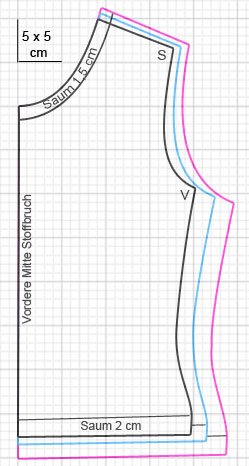
\includegraphics[width=64.54mm]{Front.jpg}
      \caption{Front Pattern}
      \label{fig:Front}
\end{figure}

These are the sample equations for the design
% For single equations
\begin{equation}
 b = h + t\\
\end{equation}

% This is the code for multiple equation
\begin{eqnarray}
%if you want no number to the equation then use \nonumber
a & = & b + c \\
& = & d + e \\
& = & f + g 
\end{eqnarray}
%%%%%%%

%%%%%%%
\subsubsection{Back}

for the back portion all the details are written here

\begin{figure}[ht!]
     \centering
     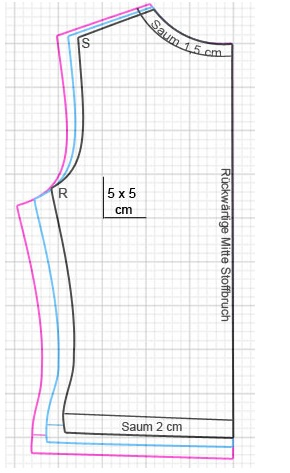
\includegraphics[width=64.54mm]{Back_pattern.jpg}
      \caption{Back Pattern}
      \label{fig:Back}
\end{figure}

These are the equations for back portion
% For single equations
\begin{equation}
 b = h + t\\
\end{equation}


% This is the code for multiple equation
\begin{eqnarray}
%if you want no number to the equation then use \nonumber
a & = & b + c \\
& = & d + e \\
& = & f + g
\end{eqnarray}
%%%%%%%

%%%%%%%
\subsubsection{Sleeve}

for the sleeve portion all the details are written here

\begin{figure}[ht!]
     \centering
     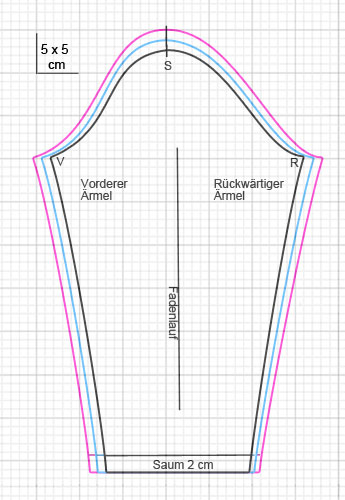
\includegraphics[width=64.54mm]{Sleeve.jpg}
      \caption{Sleeve Pattern}
      \label{fig:Sleeve}
\end{figure}

% For single equations
\begin{equation}
 b = h + t\\
\end{equation}

% This is the code for multiple equation
\begin{eqnarray}
%if you want no number to the equation then use \nonumber
a & = & b + c \\
& = & d + e \\
& = & f + g
\end{eqnarray}
%%%%%%%

%%%%%%
\subsection{Figure Captions}

See figure~\ref{fig:Front} on page~\pageref{fig:Front}.
%%%%%%%

%%%%%%%
\subsection{Table Captions}

See table~\ref{tab:Table 1} for the detailed analysis
%%%%%%%

%%%%%%%
\subsection{Page Numbers, Headers and Footers}

Page numbers, headers and footers must not be used.
%%%%%%%

%%%%%%%
\subsection{References}
for the citation of the reference use \cite{ref2}
%%%%%%%

%%%%%%%
\section{Conclusion}

for entering the conclusion
%%%%%%%

%%%%%%%
\section*{Acknowledgment}
We would like to thank Dr.Prasenjit Saha for the extremely useful discussions.
%%%%%%%

%%%%%%%
\begin{thebibliography}{99}
\bibitem{ref1} H.~Partl:
\emph{German \TeX},
TUGboat Volume~9, Issue~1 (1988)

\bibitem{ref2} H.~Part2:
\emph{German \TeX},
TUGboat Volume~9, Issue~3 (1998)

\end{thebibliography}
%%%%%%%

\end{document}
